% ---------------------------------------------------
% ----- Appendix of the template
% ----- for Bachelor-, Master thesis and class papers
% ---------------------------------------------------
%  Created by C. Müller-Birn on 2012-08-17, CC-BY-SA 3.0.
%  Freie Universität Berlin, Institute of Computer Science, Human Centered Computing. 
%

\chapter{Appendix}
\label{ch:Appendix}

\begin{figure}[t]
	\centering
	\includegraphics[angle=90,origin=c,width=330px]{/home/tim/HCC/IKON-backend/src/topicextraction/nlp/nlpflowchart_old}
	\caption{\label{pic:IKON_pipeline} BPMN process diagram of the existing topic modeling pipeline}
\end{figure}

\subsection{Protocol of the cognitive walkthrough}
{\fontsize{11}{13}\selectfont
	\begin{enumerate}
		\item Step
		\begin{itemize}
			\item \textit{Which action was selected?} \\
			2
			\item \textit{What effect was the user trying to achieve by selecting this action?} \\
			The user sees the visualization for the first time and tries to connect the cluster top words, which are displayed above the visualization and the clusters in the visualization. 
			\item \textit{How did the user know that this action was available?} \\
			This action follows from the immediate presentation of top words and scatter plot. 
			\item \textit{Did the selected action achieve the desired effect?} \\
			The user deduces that all the projects can be clustered into three clusters - a taxonomic cluster, one connected to ecosystems and one concerned with evolution. 
			\item \textit{When the action was selected, could the user determine how things were going?} \\
			This action did not change the visualization.
			\item \textit{Which explainability technique was used?}\\
			Top words
		\end{itemize}
		\begin{figure}[H]
			\centering
			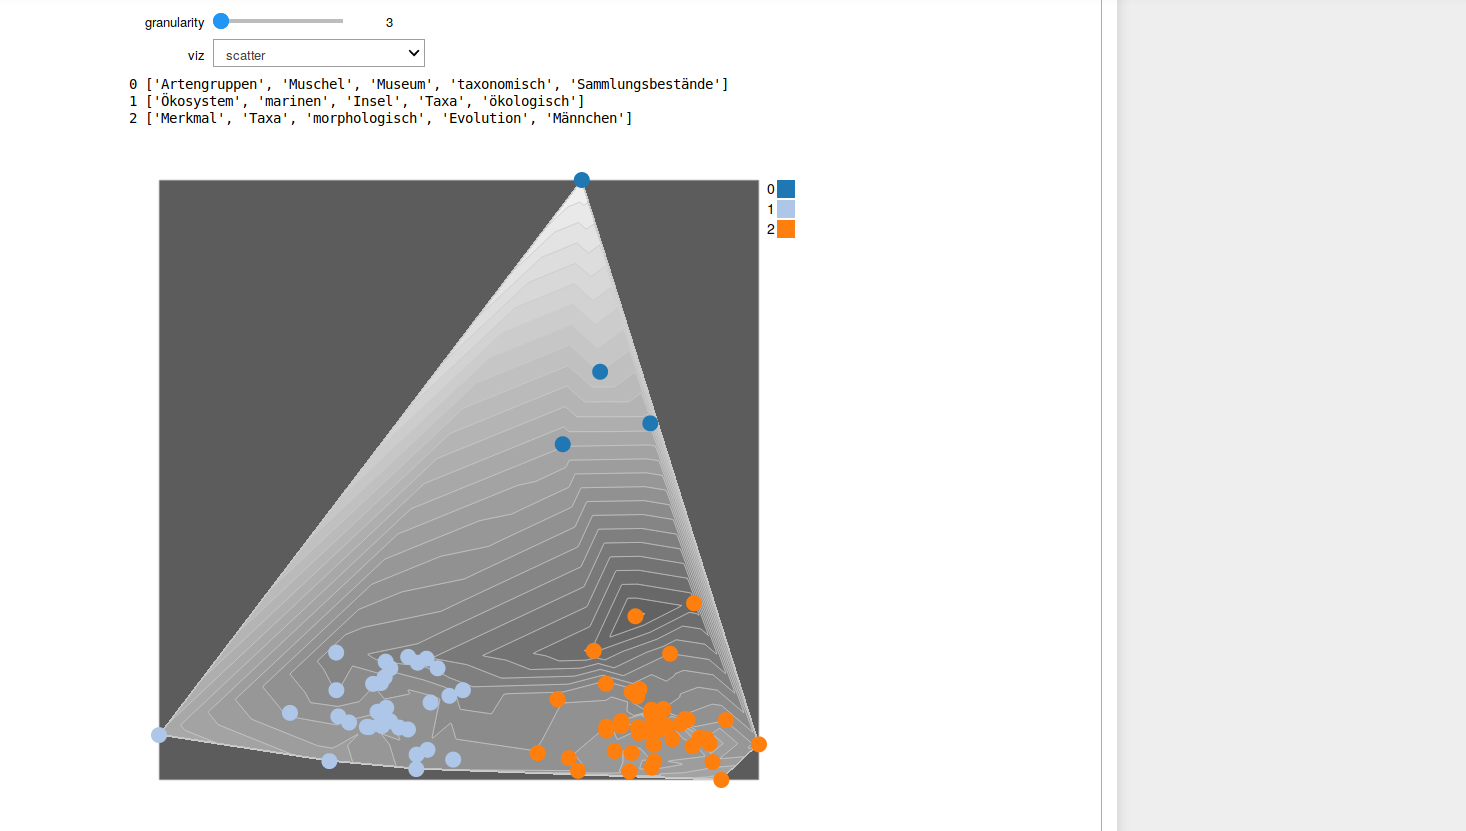
\includegraphics[width=390px]{../chapters/validation/pics/1_c}
			\caption{\label{pic:step1} Cognitive Walkthrough step 1}
		\end{figure} \newpage
		
		\item Step
		\begin{itemize}
			\item \textit{Which action was selected?} \\
			3
			\item \textit{What effect was the user trying to achieve by selecting this action?} \\
			The user concluded that his project must be in the 'evolution' cluster and therefore he changes the granularity by moving the slider to the middle of the selection range. 
			\item \textit{How did the user know that this action was available?} \\
			It was the only available slider and its label suggested that this is the proper action. 
			\item \textit{Did the selected action achieve the desired effect?} \\
			The user sees a more granular clustering over all projects. 
			\item \textit{When the action was selected, could the user determine how things were going?} \\
			Since there is no transition, the user does not know what is happening.
			\item \textit{Which explainability technique was used?}\\
			Top words
		\end{itemize}
		\begin{figure}[H]
			\centering
			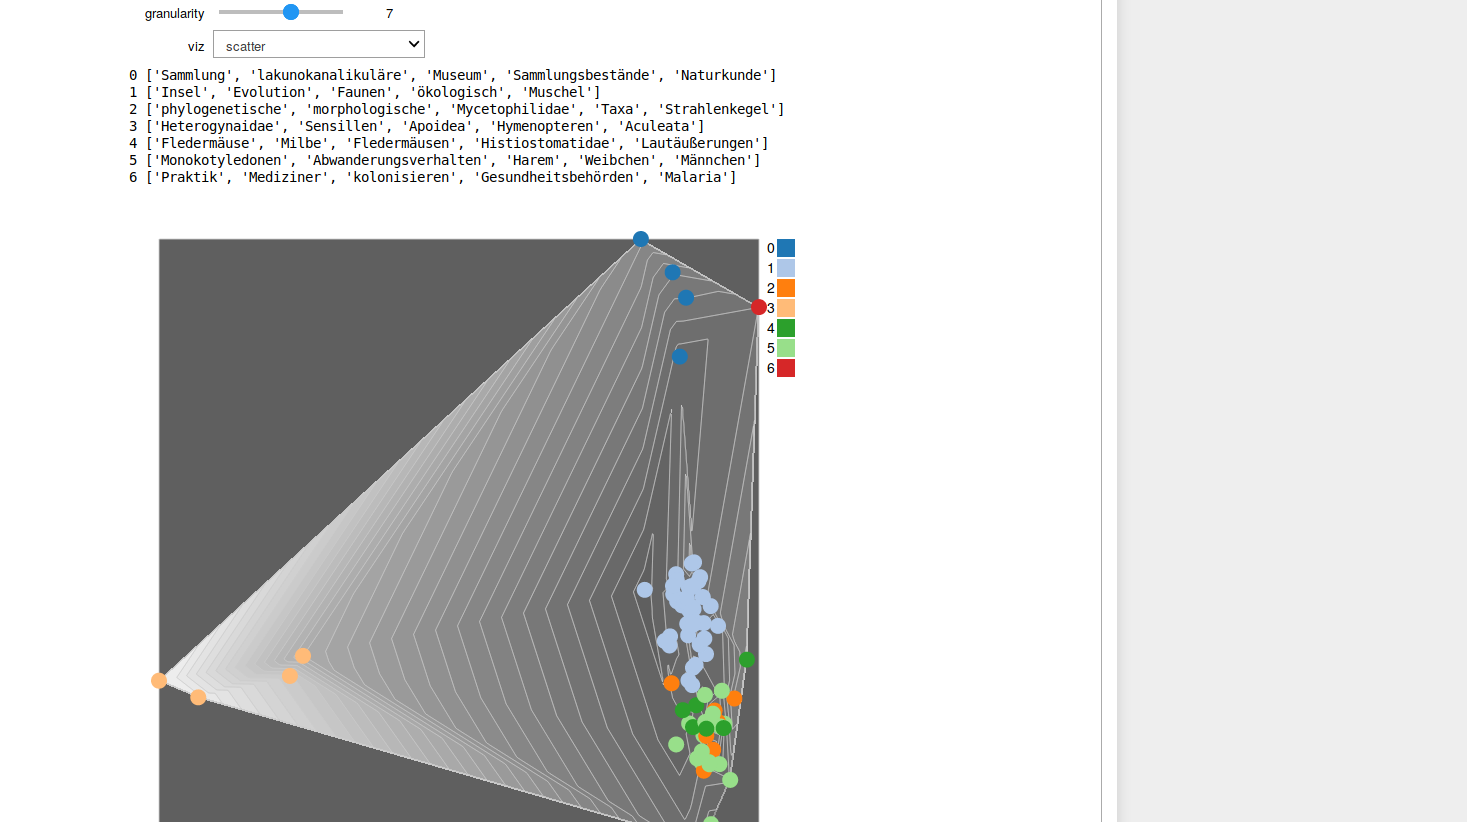
\includegraphics[width=400px]{../chapters/validation/pics/2_c}
			\caption{\label{pic:step2} Cognitive Walkthrough step 2}
		\end{figure} \newpage
		
		\item Step
		\begin{itemize}
			\item \textit{Which action was selected?} \\
			2
			\item \textit{What effect was the user trying to achieve by selecting this action?} \\
			After changing the granularity, the user is trying to pinpoint the cluster to which his project is now assigned. 
			\item \textit{How did the user know that this action was available?} \\
			As in the beginning the immediate presentation of the topwords and the visualization makes it inevitable to read and connect both. 
			\item \textit{Did the selected action achieve the desired effect?} \\
			The user determined that his project is probably in cluster 4. 
			\item \textit{When the action was selected, could the user determine how things were going?} \\
			This action did not change the visualization.
			\item \textit{Which explainability technique was used?}\\
			None
		\end{itemize}
		\begin{figure}[H]
			\centering
			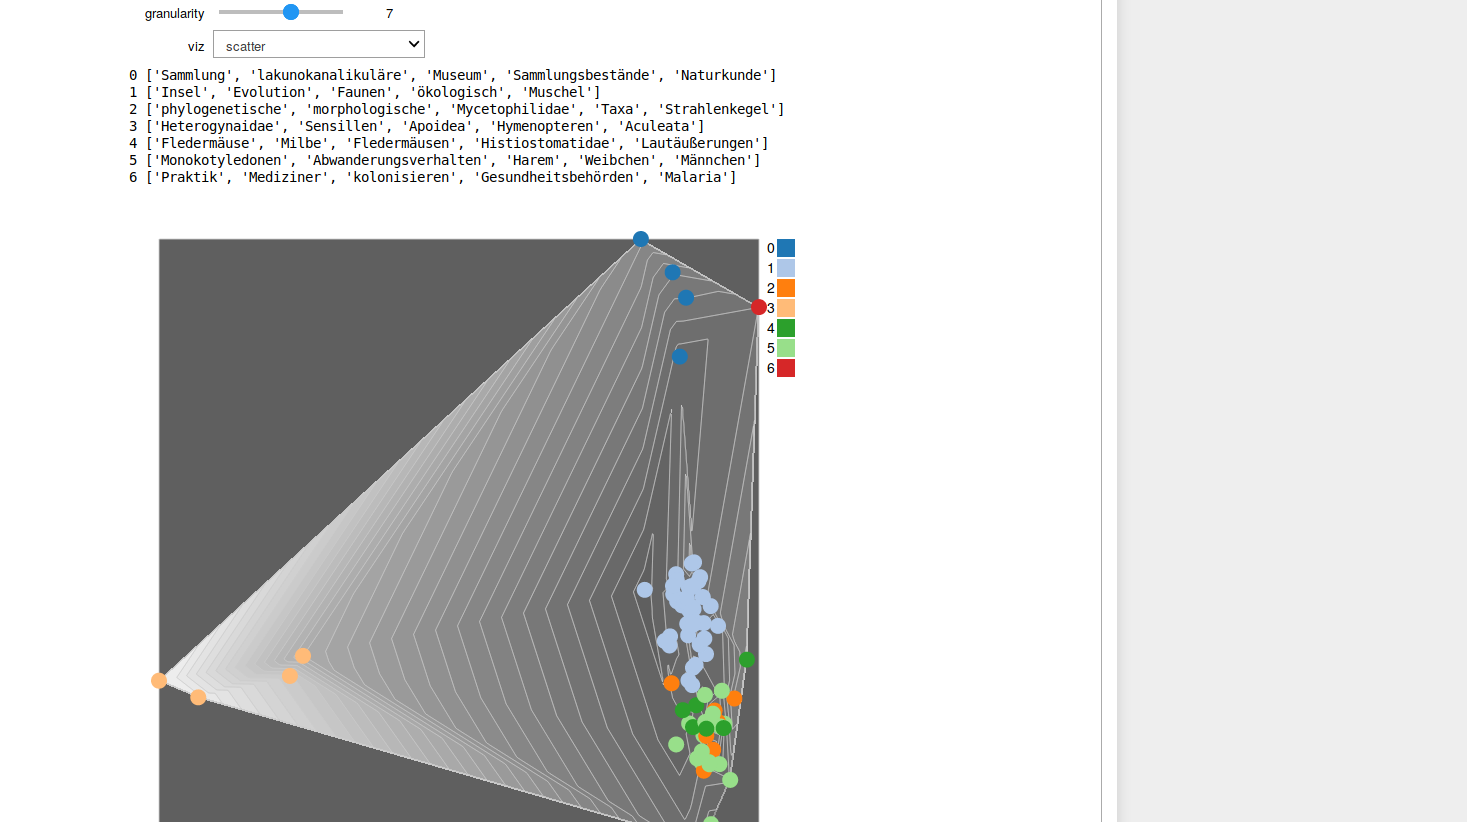
\includegraphics[width=400px]{../chapters/validation/pics/2_c}
			\caption{\label{pic:step3} Cognitive Walkthrough step 3}
		\end{figure} \newpage
		
		\item Step
		\begin{itemize}
			\item \textit{Which action was selected?} \\
			1
			\item \textit{What effect was the user trying to achieve by selecting this action?} \\
			The user is trying to find his project in cluster 4. 
			\item \textit{How did the user know that this action was available?} \\
			Hovering over a glyph to display metadata is a common design strategy and therefore the user tried this first. 
			\item \textit{Did the selected action achieve the desired effect?} \\
			The selected project was not the correct one. 
			\item \textit{When the action was selected, could the user determine how things were going?} \\
			Since the metadata is displayed right alongside the project and the rest didn't change, there was no confusion.
			\item \textit{Which explainability technique was used?}\\
			Top words
		\end{itemize}
		\begin{figure}[H]
			\centering
			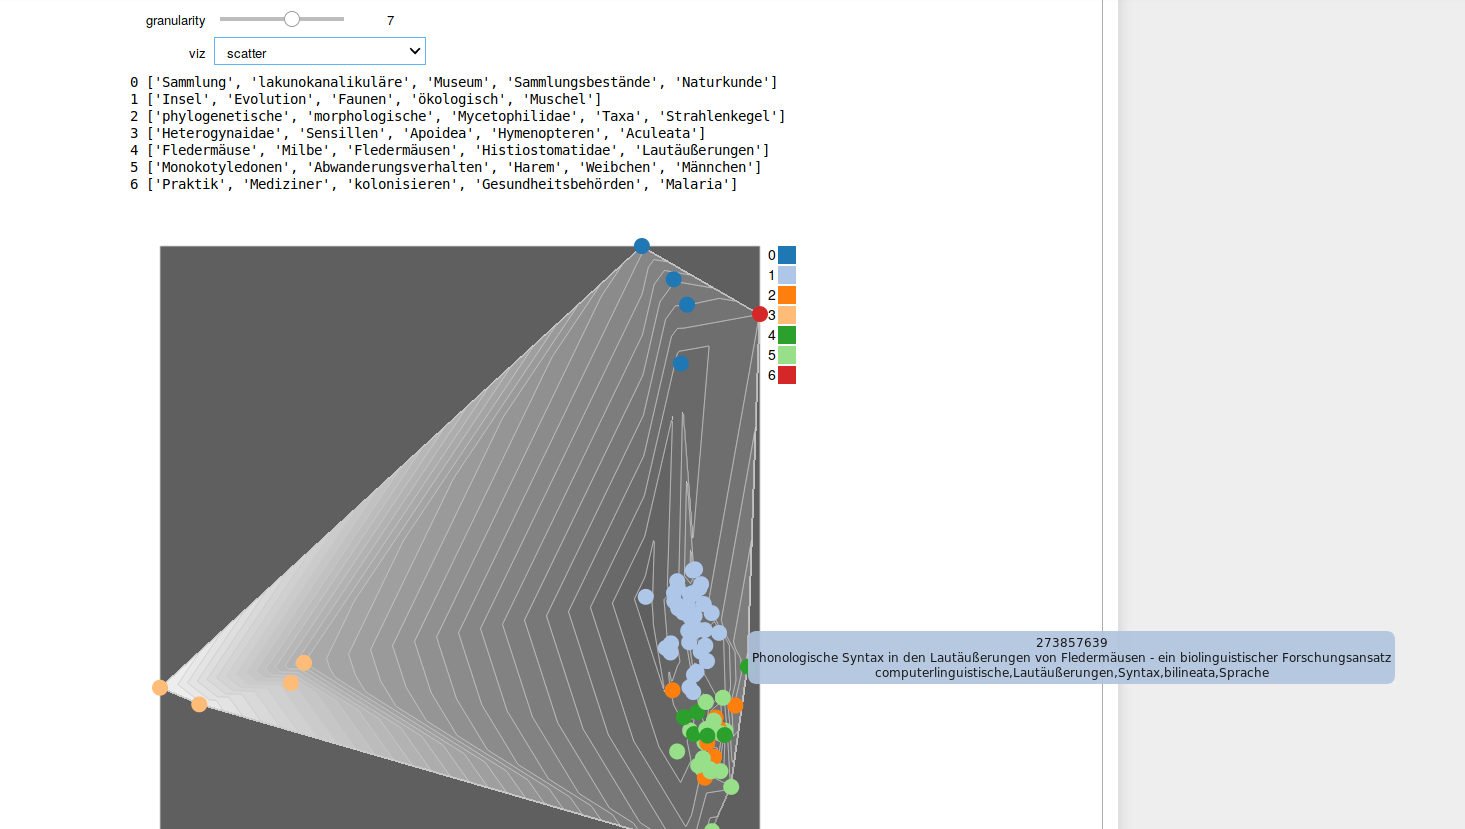
\includegraphics[width=400px]{../chapters/validation/pics/3_c}
			\caption{\label{pic:step4} Cognitive Walkthrough step 4}
		\end{figure} \newpage
		
		\item Step
		\begin{itemize}
			\item \textit{Which action was selected?} \\
			1
			\item \textit{What effect was the user trying to achieve by selecting this action?} \\
			The user is trying to find his project in cluster 4. 
			\item \textit{How did the user know that this action was available?} \\
			Hovering over a glyph to display metadata is a common design strategy and therefore the user tried this first. 
			\item \textit{Did the selected action achieve the desired effect?} \\
			The selected project was again not the correct one. 
			\item \textit{When the action was selected, could the user determine how things were going?} \\
			Since the metadata is displayed right alongside the project and the rest didn't change, there was no confusion.
			\item \textit{Which explainability technique was used?}\\
			Top words
		\end{itemize}
		\begin{figure}[H]
			\centering
			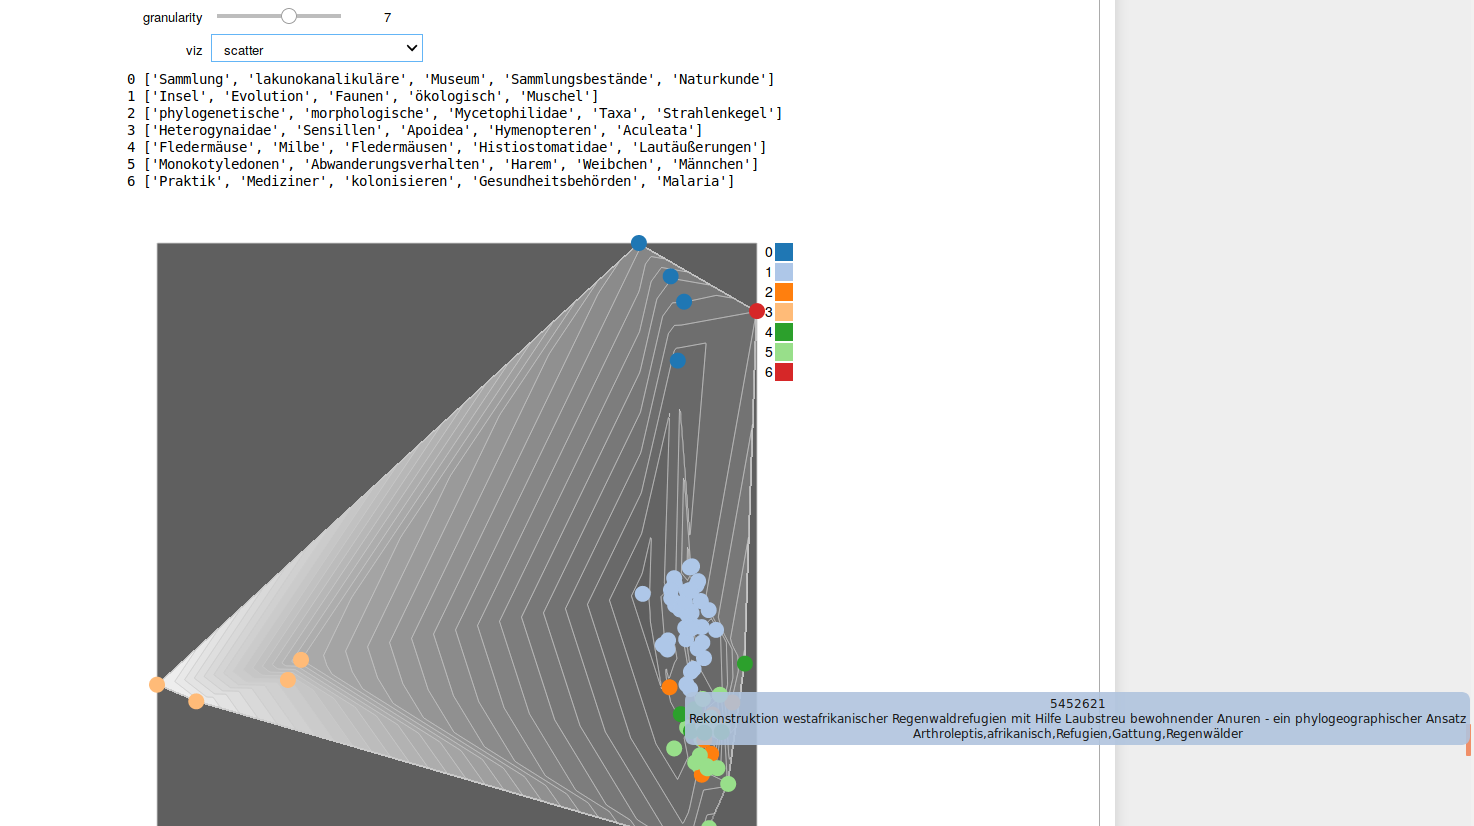
\includegraphics[width=400px]{../chapters/validation/pics/4_c}
			\caption{\label{pic:step5} Cognitive Walkthrough step 5}
		\end{figure} \newpage
		
		\item Step
		\begin{itemize}
			\item \textit{Which action was selected?} \\
			4
			\item \textit{What effect was the user trying to achieve by selecting this action?} \\
			Since the rest of the cluster is extremely cluttered, the user decides to switch into the linearized view 
			\item \textit{How did the user know that this action was available?} \\
			This is the only remaining interaction option, but the naming of this selection makes it hard to intuitivly understand what it does. 
			\item \textit{Did the selected action achieve the desired effect?} \\
			The scatter plot got uncluttered by linearization. 
			\item \textit{When the action was selected, could the user determine how things were going?} \\
			Since there is no animated transition, the user does not really know how the scatter plot and this view are connected. Furthermore the cluster assignments and the top words changed, because the whole pipeline was computed from ground up. This adds into the confusion.
			\item \textit{Which explainability technique was used?}\\
			Linearization
		\end{itemize}
		\begin{figure}[H]
			\centering
			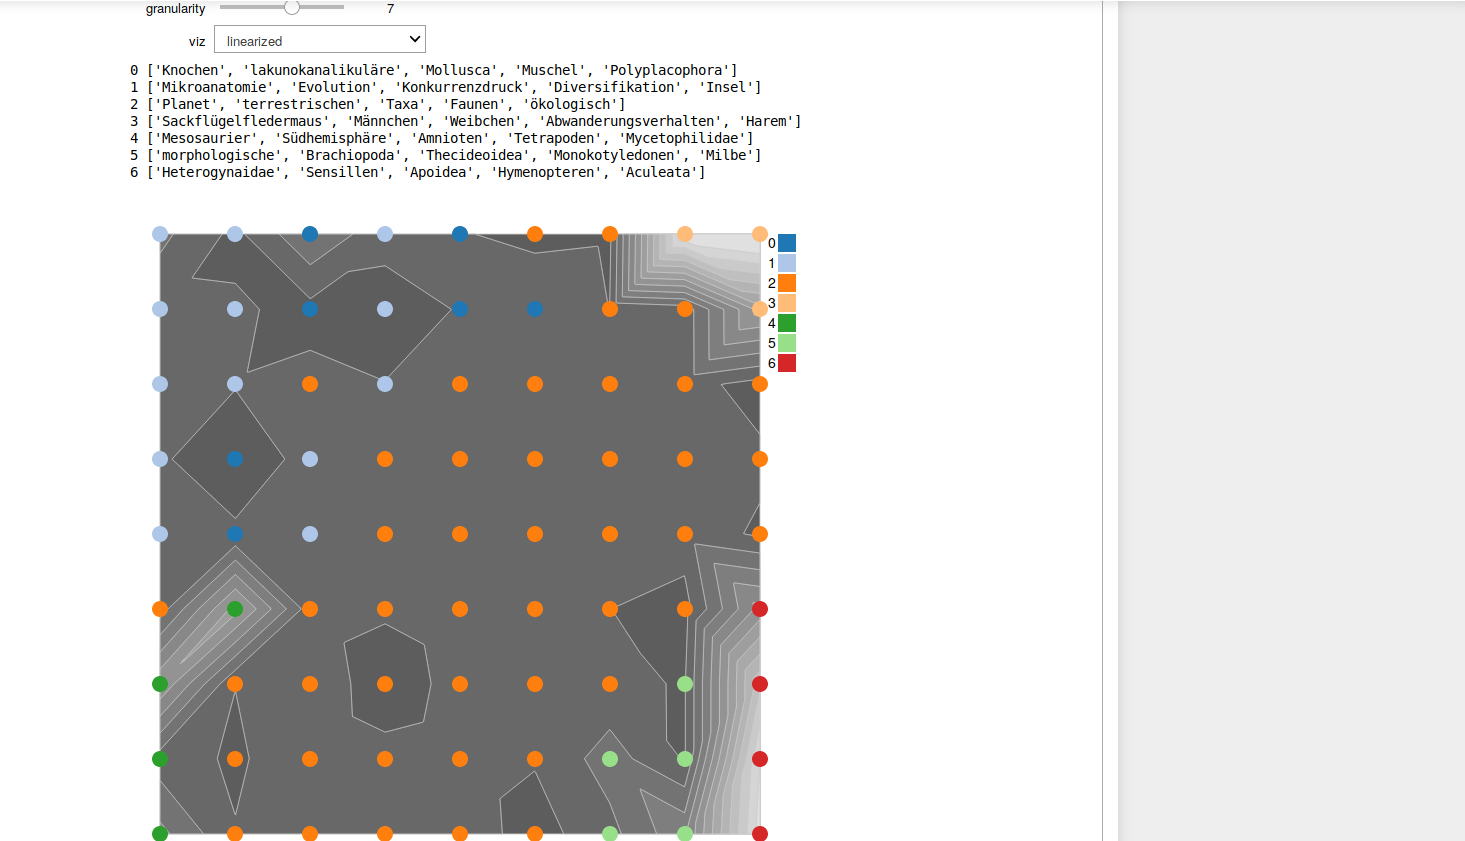
\includegraphics[width=400px]{../chapters/validation/pics/5_c}
			\caption{\label{pic:step6} Cognitive Walkthrough step 6}
		\end{figure} \newpage
		
		\item Step
		\begin{itemize}
			\item \textit{Which action was selected?} \\
			2
			\item \textit{What effect was the user trying to achieve by selecting this action?} \\
			Now that the clustering and assignments changed again, the user is again searching for the cluster in which his project may lie. 
			\item \textit{How did the user know that this action was available?} \\
			As in the previous instances of this action this is the only available, logical action. 
			\item \textit{Did the selected action achieve the desired effect?} \\
			The user is able to pinpoint cluster 3 as the cluster connected to bats. 
			\item \textit{When the action was selected, could the user determine how things were going?} \\
			Nothing changed, therefore there was no room for confusion.
			\item \textit{Which explainability technique was used?}\\
			Top words
		\end{itemize}
		\begin{figure}[H]
			\centering
			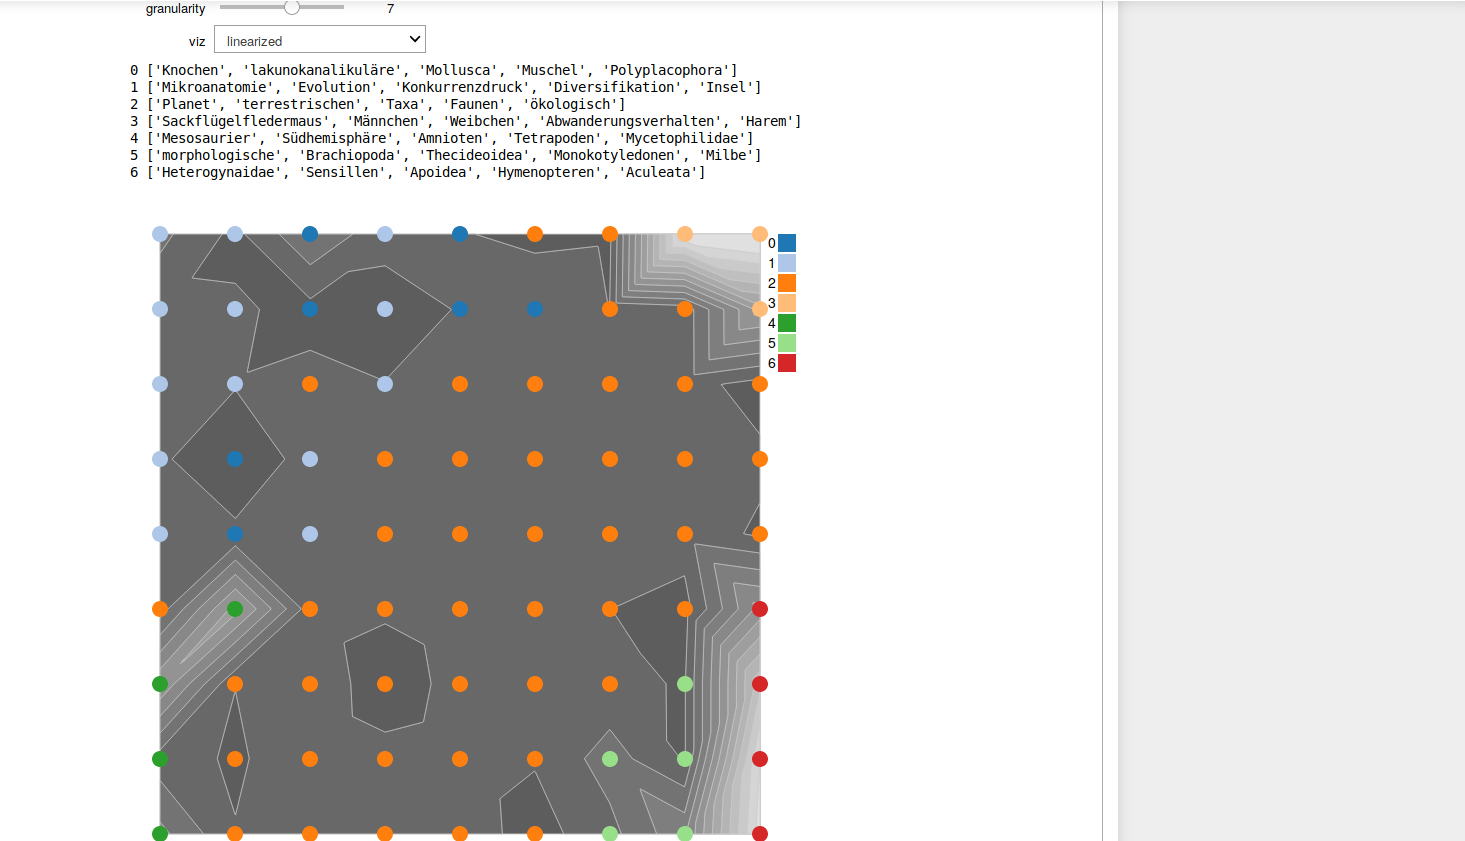
\includegraphics[width=400px]{../chapters/validation/pics/5_c}
			\caption{\label{pic:step7} Cognitive Walkthrough step 7}
		\end{figure} \newpage
		
		\item Step
		\begin{itemize}
			\item \textit{Which action was selected?} \\
			1
			\item \textit{What effect was the user trying to achieve by selecting this action?} \\
			The user is searching for his project and selects the first visible glyph. 
			\item \textit{How did the user know that this action was available?} \\
			In the previous steps the user verified that hovering for metadata is a possibility. 
			\item \textit{Did the selected action achieve the desired effect?} \\
			The project he selected was indeed his own project. All of the top words make sense in the context of his project. 
			\item \textit{When the action was selected, could the user determine how things were going?} \\
			Again there was no confusion.
			\item \textit{Which explainability technique was used?}\\
			Top words
		\end{itemize}
		\begin{figure}[H]
			\centering
			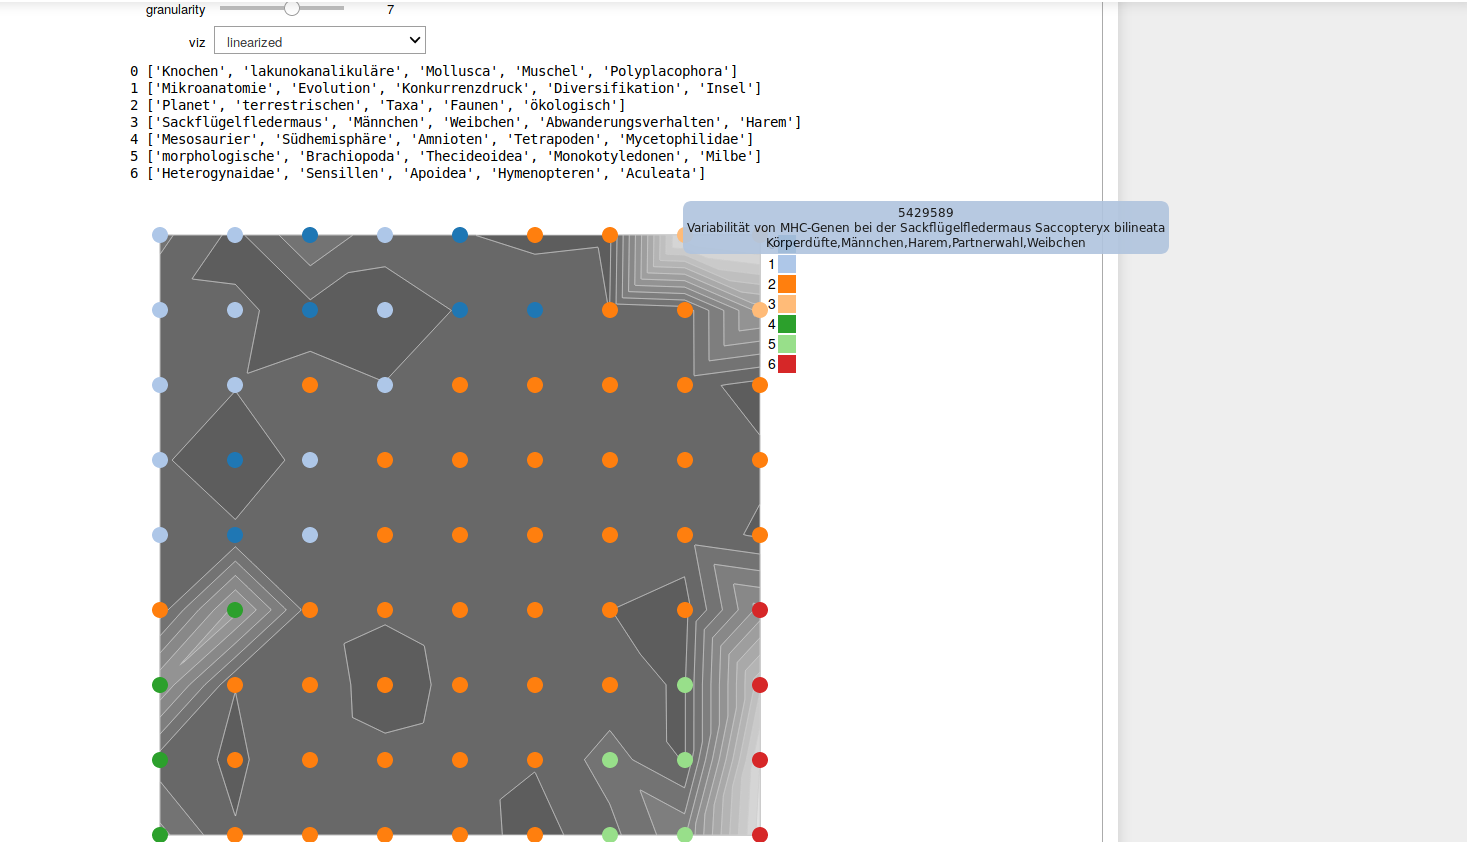
\includegraphics[width=400px]{../chapters/validation/pics/6_c}
			\caption{\label{pic:step8} Cognitive Walkthrough step 8}
		\end{figure} \newpage
		
		\item Step
		\begin{itemize}
			\item \textit{Which action was selected?} \\
			1
			\item \textit{What effect was the user trying to achieve by selecting this action?} \\
			Now that he found his project the user is interested what kind of projects are also in the cluster which was assigned to his project. Therefore he selects the next available project in the same cluster. 
			\item \textit{How did the user know that this action was available?} \\
			In the previous steps the user verified that hovering for metadata is a possibility. 
			\item \textit{Did the selected action achieve the desired effect?} \\
			The next project is also connected to the very same research subject. Therefore the clustering makes sense and the top words also are closely related to the top words of his own project. 
			\item \textit{When the action was selected, could the user determine how things were going?} \\
			Again there was no confusion.
			\item \textit{Which explainability technique was used?}\\
			Top words
		\end{itemize}
		\begin{figure}[H]
			\centering
			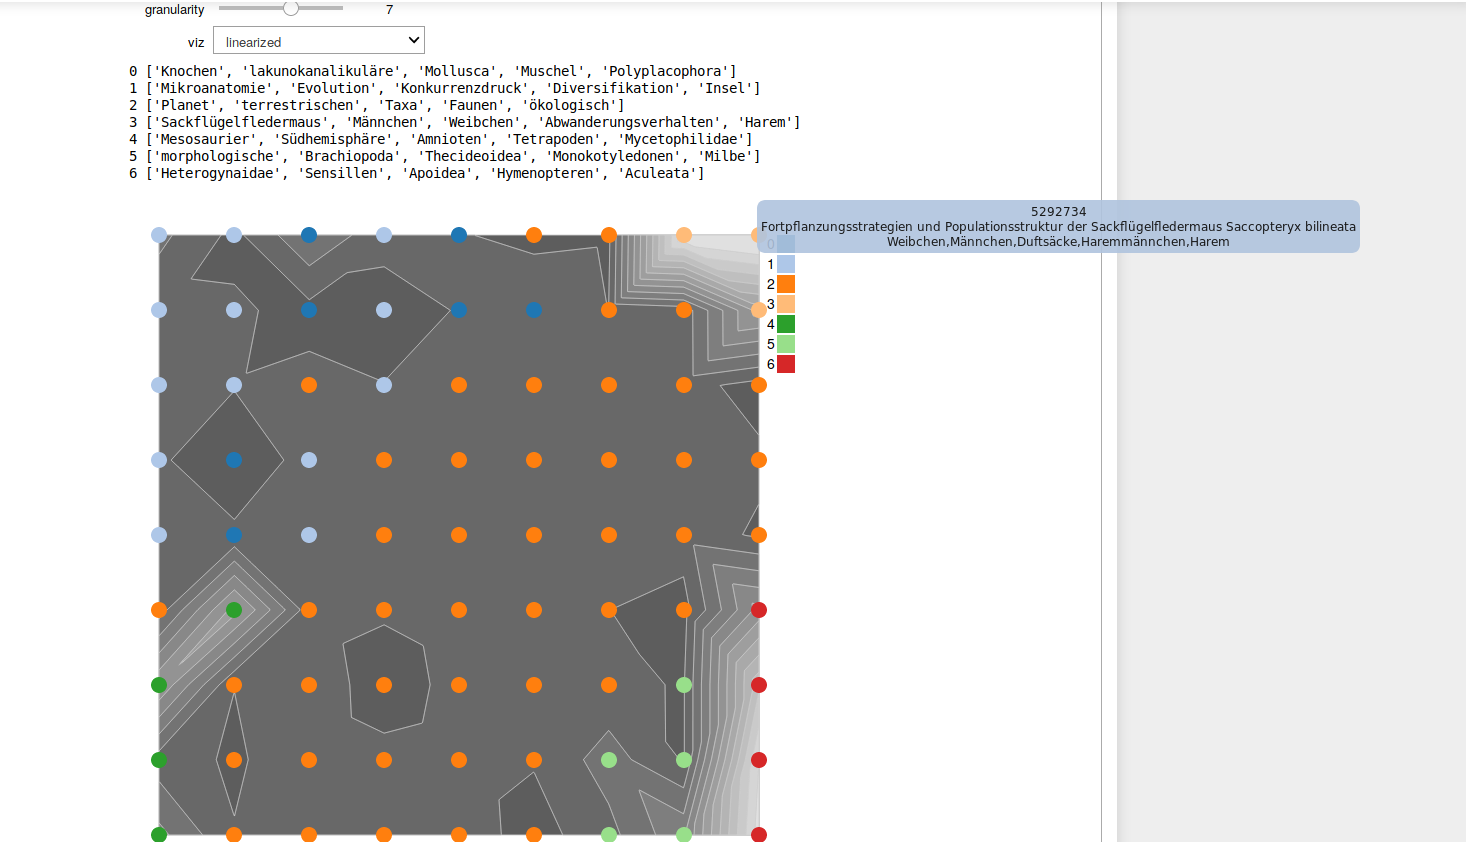
\includegraphics[width=400px]{../chapters/validation/pics/7_c}
			\caption{\label{pic:step9} Cognitive Walkthrough step 9}
		\end{figure} \newpage
		
		\item Step
		\begin{itemize}
			\item \textit{Which action was selected?} \\
			1
			\item \textit{What effect was the user trying to achieve by selecting this action?} \\
			The user selects the last remaining project in the same cluster to see if it also fits into the cluster since the topography suggests that it may fit less well into the overarching topic. 
			\item \textit{How did the user know that this action was available?} \\
			In the previous steps the user verified that hovering for metadata is a possibility. 
			\item \textit{Did the selected action achieve the desired effect?} \\
			The last project is also connected to a similar research subject, although it differs a bit due to it rather being concerned with migration of bats than procreation. Since the topwords also suggest this, it further validates the clustering. 
			\item \textit{When the action was selected, could the user determine how things were going?} \\
			Again there was no confusion.
			\item \textit{Which explainability technique was used?}\\
			Top words, Cluster Topography
		\end{itemize}
		\begin{figure}[H]
			\centering
			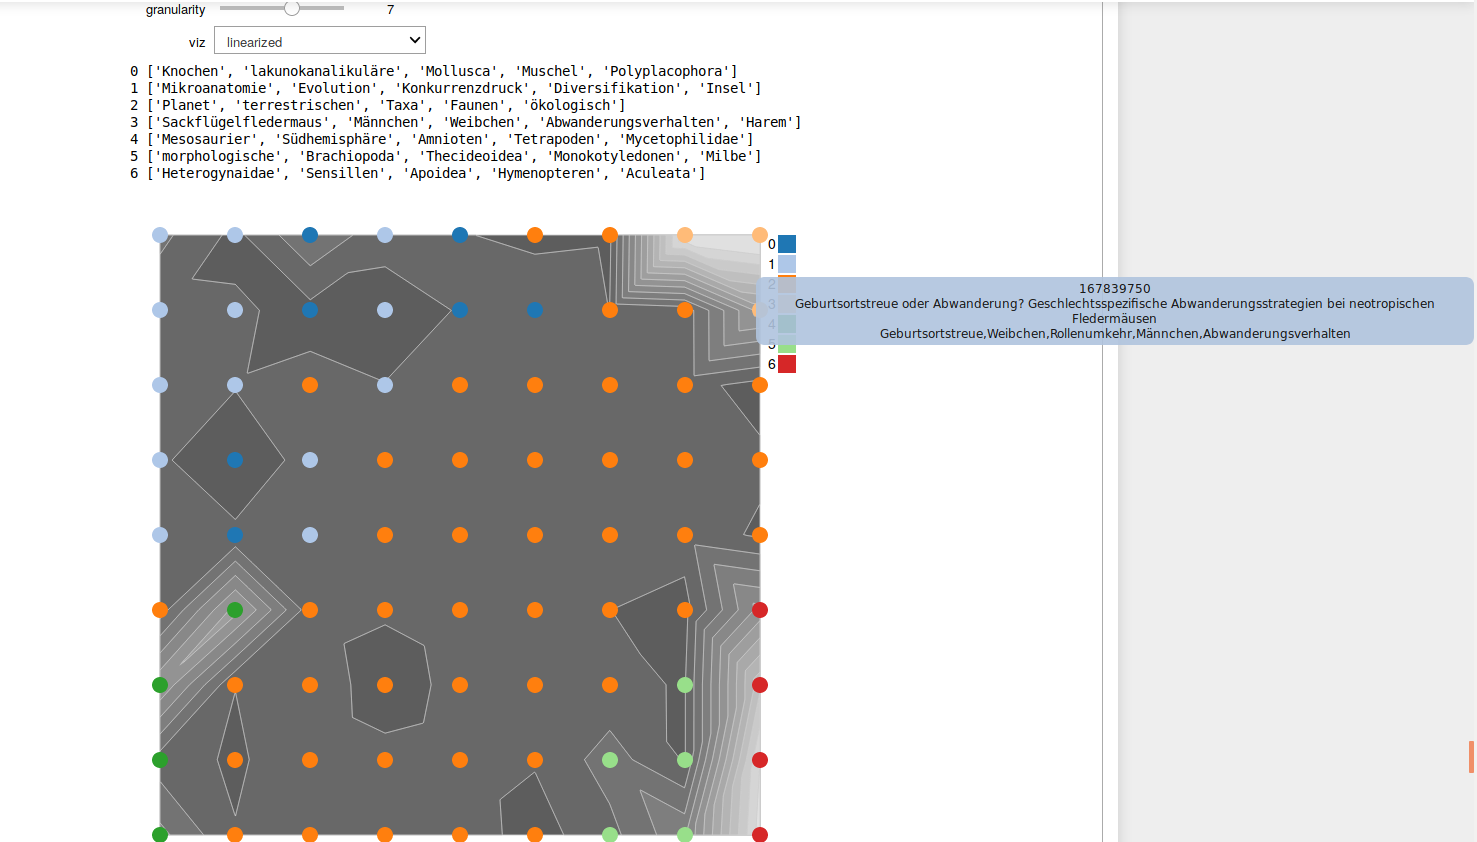
\includegraphics[width=400px]{../chapters/validation/pics/8_c}
			\caption{\label{pic:step10} Cognitive Walkthrough step 10}
		\end{figure} \newpage
		
		\item Step
		\begin{itemize}
			\item \textit{Which action was selected?} \\
			1
			\item \textit{What effect was the user trying to achieve by selecting this action?} \\
			Since the cluster does make sense the user decides to have a look at the neighbouring projects. Especially since the selected one seems to fit worse into its cluster than the rest. 
			\item \textit{How did the user know that this action was available?} \\
			In the previous steps the user verified that hovering for metadata is a possibility. 
			\item \textit{Did the selected action achieve the desired effect?} \\
			The first project he selects does investigate a completly different field. 
			\item \textit{When the action was selected, could the user determine how things were going?} \\
			The user is able to tell why the project lies in another cluster using the top words.
			\item \textit{Which explainability technique was used?}\\
			Top words, Cluster topography
		\end{itemize}
		\begin{figure}[H]
			\centering
			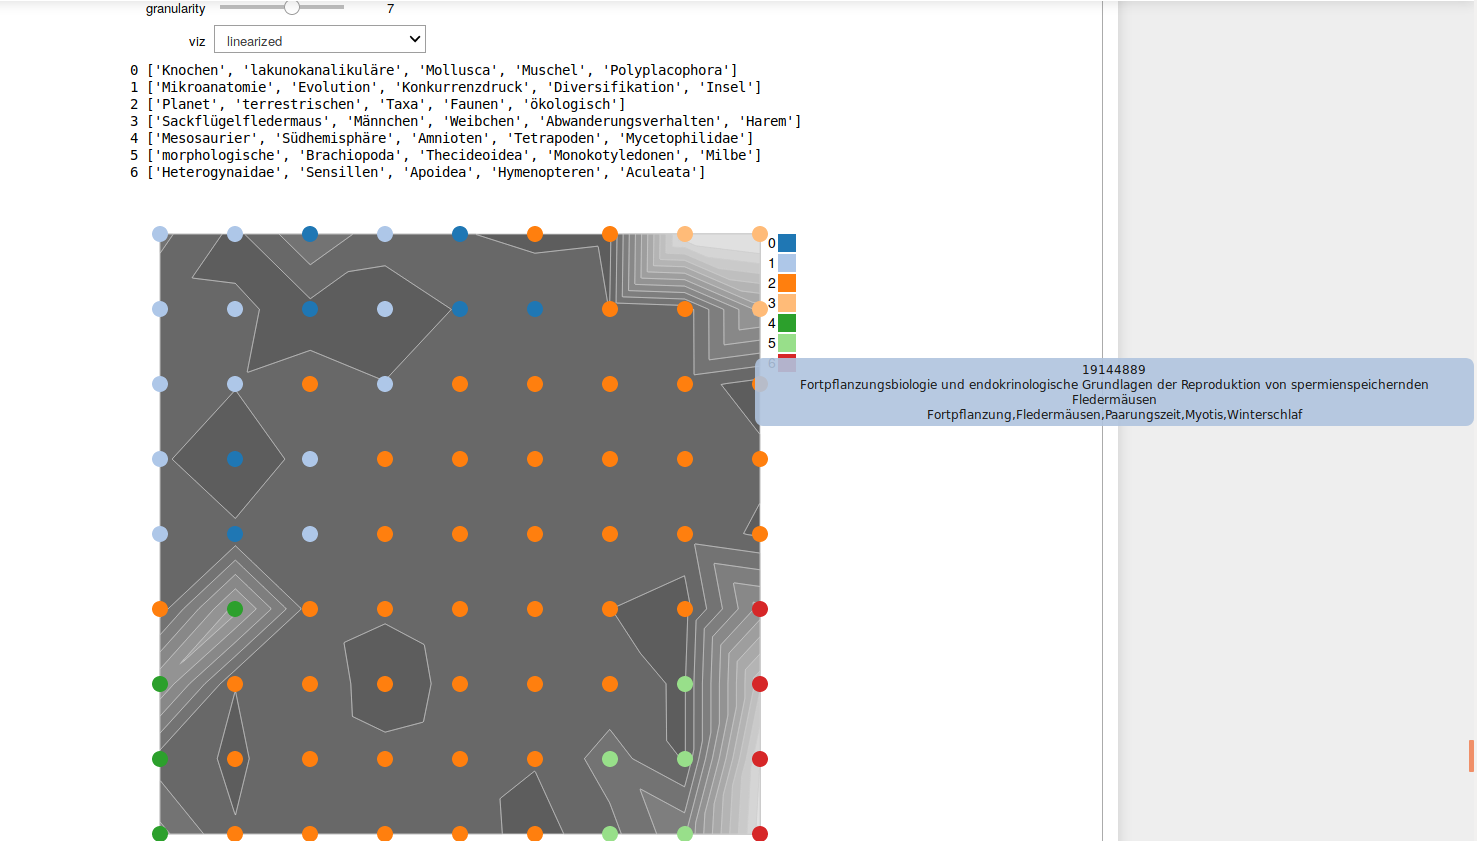
\includegraphics[width=400px]{../chapters/validation/pics/9_c}
			\caption{\label{pic:step11} Cognitive Walkthrough step 11}
		\end{figure} \newpage
		
		\item Step
		\begin{itemize}
			\item \textit{Which action was selected?} \\
			1
			\item \textit{What effect was the user trying to achieve by selecting this action?} \\
			The user still thinks that there may be another similar project, because the top words of cluster 2 are a concerned with ecology, faunas and taxonomies. 
			\item \textit{How did the user know that this action was available?} \\
			In the previous steps the user verified that hovering for metadata is a possibility. 
			\item \textit{Did the selected action achieve the desired effect?} \\
			The next project he selects is surprisingly also connected to bats.  
			\item \textit{When the action was selected, could the user determine how things were going?} \\
			The user is not entirely sure why this project was not categorized in his own cluster. The top words suggest that the work is rather specialzed on the biological processes of procreation using bats as a use case. 
			\item \textit{Which explainability technique was used?}\\
			Top words
		\end{itemize}
		\begin{figure}[H]
			\centering
			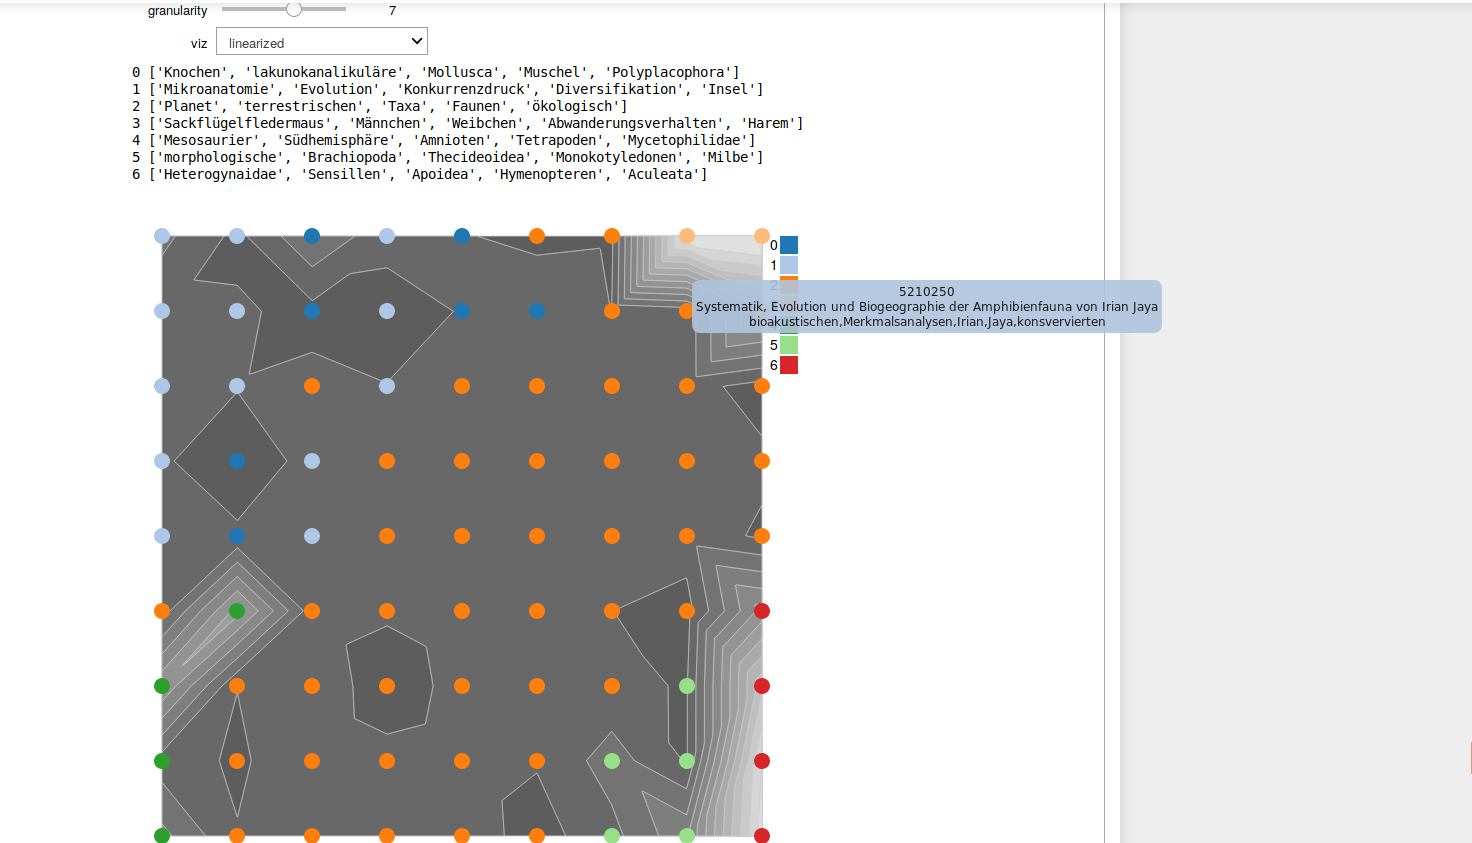
\includegraphics[width=400px]{../chapters/validation/pics/10_c}
			\caption{\label{pic:step12} Cognitive Walkthrough step 12}
		\end{figure}
\end{enumerate}}

